

\Gls{snn} ieejas dati jākodē kā retu impulsu virknes, lai tie atbilstu impulsu neironu darbībai laikā. Tā vietā, lai
katrā laika solī pārraidītu visu neironu stāvokļus, tiek pārraidīti tikai neironi, kas ģenerē impulsu. Tas būtiski
samazina pārsūtāmo datu apjomu, ja impulsu aktivitāte ir reta. Vairumā gadījumu izmanto saspiestu \Gls{aer} reprezentāciju
\cite{sommer2022, plagwitz2025}, kas efektīvi kodē impulsu aktivitāti kā diskrētas notikumu adreses telpā un laikā.

Kā ilustrēts \ref{fig:aer_comm}. attēlā, kad neirons ģenerē impulsu, tā telpiskā pozīcija tiek kodēta adresē un pārraidīta pa sakaru kanālu. Uztvērējā adrese tiek dekodēta, lai atjaunotu impulsa notikumu. Tā kā impulsus ģenerē tikai aktīvie neironi, sakaru joslas platums mainās atkarībā no impulsu skaita, nevis neironu skaita \cite{purohit2022}.

\begin{figure}[!t]
  \centering
  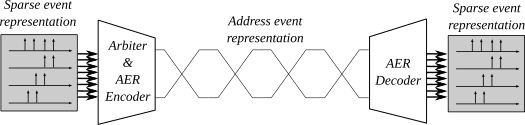
\includegraphics[width=0.8\linewidth]{fig/aer_encoder_decoder.png}
  \caption{AER saziņa.}
  \label{fig:aer_comm}
% \par\smallskip
% {\footnotesize \textit{Sparse event representation} — retināta notikumu reprezentācija; \textit{Arbiter \& AER Encoder} — arbitrs un AER kodētājs; \textit{Address event representation} — adrešu un notikumu reprezentācija; \textit{AER Decoder} — AER dekodētājs.\par}
\end{figure}

Šajā darbā tradicionālais \Gls{aer} protokols ir paplašināts, lai reprezentētu konvolucionālo \Gls{snn} slāņu radītās daudzkanālu pazīmju kartes. Saskaņā ar šo kodēšanas shēmu katru impulsu attēlo viena vesela skaitļa adrese, kas veidota, bitu līmenī savienojot telpiskos un kanāla indeksus, kā parādīts \ref{fig:aer_bits}. attēlā. Precīzāk, katra impulsa adrese \(a\) tiek kodēta kā bitu lauks:
\begin{equation}
    a[t] = (x \ll (b_h + b_c + 1)) | (y \ll (b_c + 1)) | (c \ll 1) | l,
\end{equation}
kur \(x, y\) ir 2D telpiskās koordinātas, \(c\) ir kanāla adrese un \(b_h, b_c\) ir iepriekš noteikts bitu skaits atkarībā no telpiskajām un kanālu dimensijām. Papildus \(l\) ir neobligāts jaunākās kārtas bits, ko izmanto atkārtotu vai vairāklīmeņu notikumu atšķiršanai vienā pozīcijā, ja nepieciešama reprezentācija ar vairāk nekā vienu aktīvu impulsa bitu.

\begin{figure}[!t]
  \centering
  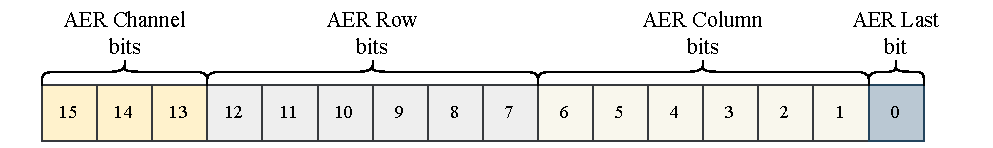
\includegraphics[width=0.8\linewidth]{fig/aer_bits.pdf}
  \caption{AER bitu lauks. Telpisko un kanāla indeksu savienošana bitu līmenī.}
  \label{fig:aer_bits}
\end{figure}

\(x, y\) vērtības nosaka, palielinot rindu un kolonnu rādītājus, līdz tiek atrasti impulsi. Pēc tam, izmantojot prioritātes kodētāju, impulsus kodē kanāla \(c\) binārā reprezentācijā, kas atbilst nozīmīgākās aktivizētās līnijas indeksam. Pilnu \Gls{aer} vārdu veido, bitu līmenī savienojot telpiskos \(x, y\) un kanāla \(c\) indeksus.

Impulsu adreses reprezentācija nodrošina efektīvāku glabāšanu un saziņu, kodējot visu nepieciešamo informāciju vienā vesela skaitļa vārdā. Kanāla indeksa reprezentācijai nepieciešamais bitu platums tiek efektīvi samazināts par \(\log_{2} N\), kur \(N\) ir vienā binārā impulsu vārdā kodēto kanālu skaits.

